\documentclass[12pt,oneside,a4paper,article]{abntex2}
\usepackage[utf8]{inputenc} % Codificação do documento
\usepackage{lmodern}
\usepackage[brazil]{babel}  % Idioma do documento
\usepackage{graphicx}       % Inclusão de gráficos
\usepackage{tabularx}       % Tabelas avançadas
\usepackage{amsmath}        % Melhorias em matemática
\usepackage{lipsum}         % Geração de texto dummy
\usepackage{authblk}
\usepackage{titlesec}
\usepackage{parskip}
\usepackage{pdfpages}
\usepackage{chngcntr,tocloft}
\usepackage{float}   

% Configurações específicas do abntex2
% Aqui você pode adicionar configurações específicas, como redefinições de comandos
% ou adições de novos pacotes que são essenciais para o seu documento.

% Carrega o pacote abntex2cite para citações
\usepackage[alf]{abntex2cite} % ou use [num] para citações numéricas

    
\usepackage[left=3cm,right=2.5cm,top=3cm,bottom=2cm]{geometry} % Margens
\usepackage{setspace}       % Espaçamento entre linhas
\usepackage{natbib}      % Formatação de bibliografia


% Informações de título
\title{\textbf{Sistema de Mapeamento para Supermercados - SuperMercado +}}
\author{Alexsandro S. de O. Júnior \thanks{alexsandro.junior@ucsal.edu.br}}
\author{Fernando Santos Barbosa \thanks{fernando.barbosa@ucsal.edu.br}}
\author{João Moraes Gordilho \thanks{joaomoraes.gordilho@edu.ucsal.br}}
\author[1]{Antonio Victor Azevedo Nascimento de Seixas Rocha \thanks{antoniovictor.rocha@ucsal.edu.br}}
\author[1]{Erivelton Madureira Lopes \thanks{erivelton.lopes@ucsal.edu.br}}
\author[1*]{Elton Figueiredo \thanks{elton.figueiredo@pro.ucsal.br}}
\affil{
    Engenharia de Software \par
    Escola de Tecnologias \par
    Universidade Católica do Salvador (UCSAL) \par
    Av. Prof. Pinto de Aguiar, 2589 Pituaçu, CEP: 41740-090 \par
    Salvador/BA, Brasil
}

\date{Setembro 2025}

\newpage

\ifthenelse{\equal{\ABNTEXisarticle}{true}}{%
\renewcommand{\maketitlehookb}{}
}{}

% Configurações de aparência do PDF final
% \usepackage{hyperref} % para inserir links
\hypersetup{
    colorlinks=false,       % false: boxed links; true: colored links
    pdfborder={0 0 0},      % remove as bordas ao redor dos links
}

\newpage
\renewcommand*{\Authsep}{, }
\renewcommand*{\Authand}{, }
\renewcommand*{\Authands}{, }
\renewcommand*{\Affilfont}{\normalsize\normalfont}
\renewcommand*{\Authfont}{\bfseries}    % make author names boldface    
\setlength{\affilsep}{2em}   % set the space between author and affiliation

\newsavebox\affbox

\counterwithin*{figure}{section}
\counterwithin*{figure}{subsection}
\counterwithin*{figure}{subsubsection}

\renewcommand{\thefigure}{%
  \ifnum\value{subsection}=0
    \thesection.\arabic{figure}%
  \else
    \ifnum\value{subsubsection}=0
      \thesubsection.\arabic{figure}%
    \else
      \thesubsubsection.\arabic{figure}%
    \fi
  \fi
}


%\usepackage[T1]{fontenc}
\renewcommand{\sfdefault}{stix} %% To make only sf fonts to be avant garde.
%\usepackage{sectsty}
%\chapterfont{\fontfamily{pag}\selectfont} %% for chapter if you want
%\sectionfont{\fontfamily{pag}\selectfont}
%\subsectionfont{\fontfamily{pag}\selectfont} 
%\subsubsectionfont{\fontfamily{pag}\selectfont}


\newpage


\begin{document}

    \begin{center}
        
\includegraphics[width=0.3\textwidth]{imagens-template/templates/ucsal_logo.png} 
    \end{center}
    {\let\newpage\relax\maketitle}
    

    \newpage
    \begin{resumoumacoluna}
    \vspace{\onelineskip}
     \hspace{4.5mm}
Este trabalho apresenta o desenvolvimento do Supermercado+, um sistema web responsivo que integra os principais supermercados de cada região do Brasil em uma única plataforma, proporcionando uma experiência de compra moderna, prática e eficiente. O Supermercado+ permite localizar produtos em tempo real por meio de um Mapa Inteligente, consultar preços e informações nutricionais instantaneamente através do Leitor de Código de Barras e realizar compras online com opção de retirada. O sistema prioriza a escalabilidade, segurança, confiabilidade e portabilidade, garantindo proteção de dados e compatibilidade com diferentes dispositivos e navegadores. A interface segue um padrão moderno e minimalista, destacando funcionalidades de fácil acesso, como scanner, mapa, lista de produtos e promovendo maior eficiência e comodidade para os usuários. 

     
    \noindent
    \\
    \textbf{Palavras-chaves}: Leitor de Código de Barras, Mapa Inteligente, informações nutricionais, Usabilidade.
    \end{resumoumacoluna}

        
    \newpage
    \tableofcontents

    
    \textual
    
    \newpage
    \section{Introdução}  
    \hspace{4.5mm}
O Supermercado+ é um aplicativo web que se destaca por integrar os principais supermercados de cada região do Brasil em uma única plataforma, oferecendo uma experiência de compra moderna e eficiente. Com o aumento da demanda por soluções digitais no varejo supermercadista, identificou-se a necessidade de um sistema que facilite a localização de produtos, forneça informações detalhadas sobre preços e dados nutricionais, e permita a realização de compras online com opção de retirada. Atualmente, os consumidores enfrentam desafios como a dificuldade de encontrar produtos rapidamente dentro do supermercado e a limitação de acesso a informações precisas, o que pode impactar negativamente a eficiência das compras e a satisfação dos usuários.
    \vspace{12mm}                                
                                   
    \section{Definição do Cliente}
    \hspace{4.5mm}
A empresa Help Technology, responsável por contratar o desenvolvimento do Sistema. A Help Technology busca  soluções inovadoras para o setor supermercadista, visando modernizar o processo de compras, aumentar a eficiência operacional e melhorar a experiência do consumidor. O cliente identifica como prioridade a digitalização do varejo, a oferta de funcionalidades que facilitem a localização de produtos, a disponibilização de informações precisas sobre preços e dados nutricionais, além da possibilidade de compras online com opção de retirada, garantindo praticidade e agilidade aos usuários. 
    \vspace{12mm}                                

      \newpage                                
    \section{Análise de Viabilidade}
    \hspace{4.5mm}
O projeto Supermercado+ consiste no desenvolvimento de um sistema de supermercado que integra os principais estabelecimentos de cada região, oferecendo funcionalidades como mapa inteligente, leitor de código de barras, consulta de preços, informações nutricionais e compras online.
\\\textbf{Viabilidade Técnica:}
O sistema será desenvolvido como uma aplicação web responsiva, compatível com diferentes navegadores e sistemas operacionais (Windows, Linux e macOS), com possibilidade de futura expansão para dispositivos móveis. A equipe possui conhecimento e experiência para implementar funcionalidades como integração com APIs externas (REST e JMS), autenticação de usuários funcionalidades de pagamento seguro.
\\\textbf{Viabilidade Econômica:}
O investimento necessário para o desenvolvimento inclui custos com mão de obra, infraestrutura de servidores e ferramentas de desenvolvimento. Considerando o potencial de uso do sistema por grandes redes de supermercados e usuários finais, espera-se que o retorno sobre investimento seja satisfatório, reduzindo custos operacionais para os estabelecimentos e aumentando a comodidade dos consumidores.
\\\textbf{Viabilidade Operacional:}
O Sistema atende à demanda de consumidores e estabelecimentos de forma prática, moderna e eficiente. A interface simples e intuitiva garante fácil navegação, enquanto funcionalidades como o mapa inteligente e o scanner de códigos proporcionam agilidade no processo de compra. A escalabilidade do sistema permite suportar grandes volumes de usuários, incluindo picos sazonais como Black Friday e promoções de feriados.
\\\textbf{Viabilidade Legal e Regulamentar:}
O sistema seguirá normas de proteção de dados, garantindo a confidencialidade das informações do usuário por meio de autenticação e backups regulares. Todos os processos de pagamento e armazenamento de dados estarão em conformidade com os termos de confiabilidade estabelecidos pelo cliente.
    \vspace{12mm}   
    
    \newpage                                
    \section{Problema}
    \hspace{4.5mm}
Os consumidores enfrentam dificuldades durante o processo de compras em supermercados, devido à falta de soluções tecnológicas que otimizem a experiência de compra. Entre os principais desafios estão a demora na localização de produtos dentro das lojas, a ausência de informações nutricionais detalhadas e a limitação de acesso a preços atualizados de forma prática. Além disso, a falta de integração entre supermercados e plataformas digitais gera obstáculos para a realização de compras online de maneira ágil e segura. Esses fatores impactam diretamente a eficiência das compras, reduzindo a praticidade para o consumidor
    \vspace{12mm}                           
    
    \section{Objetivo}
    \hspace{4.5mm}
Oferecer uma solução digital inovadora que simplifique e modernize a experiência de compras em supermercados. Tornar o processo mais prático e ágil por meio de recursos como mapa inteligente para localização de produtos, leitor de código de barras para consulta de preços e informações nutricionais, além da possibilidade de efetuar compras online com retirada no local. Contribuir para a digitalização do setor supermercadista, aproximando consumidores e estabelecimentos, ao mesmo tempo em que promove eficiência, comodidade e segurança nas transações.
    \vspace{12mm}   
    
    \newpage                                        
    \section{Entrevistas com o Cliente} 
    
    \subsection{Primeira Entrevista}
    \vspace{12mm}
    
    \subsubsection{início}
    \begin{figure}[H]
        \centering
        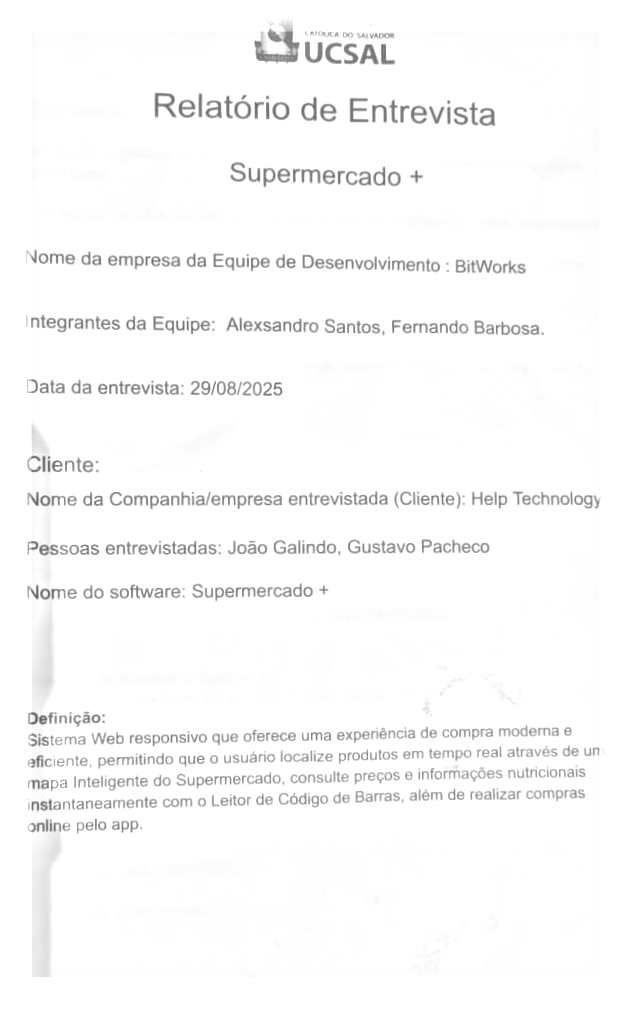
\includegraphics[width=0.75\linewidth]{imagens-template/Entrevista1/Editado4.png}
        \label{fig:placeholder}
    \end{figure}
    
  \subsubsection{Observações}
    \begin{figure}[H]
        \centering
        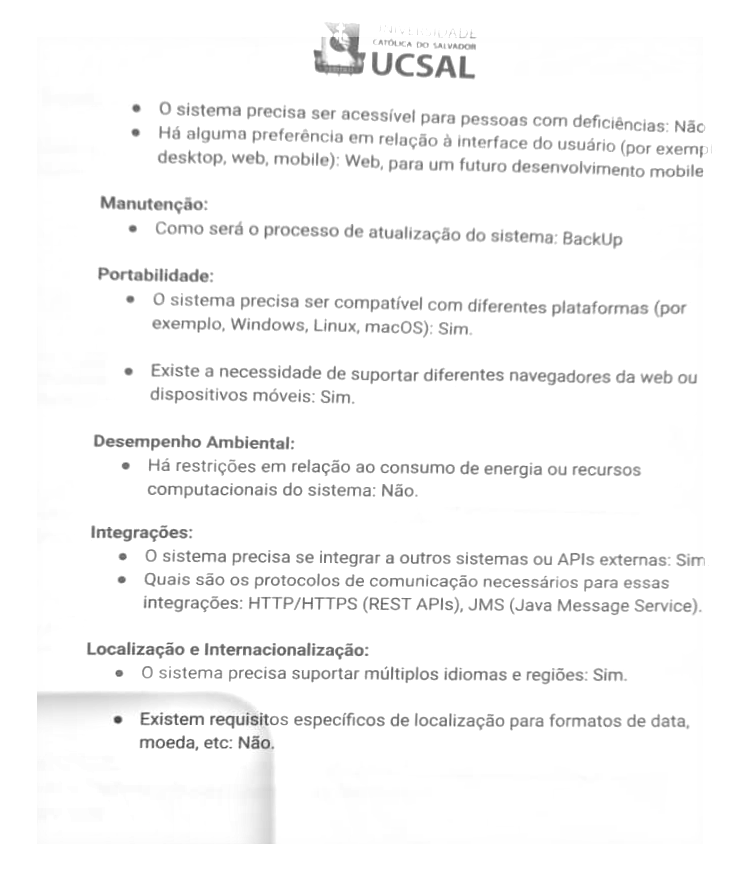
\includegraphics[width=0.75\linewidth]{imagens-template/Entrevista1/Editado3.png}
        \label{fig:placeholder}
    \end{figure}
    
  \subsubsection{Usabilidade}
    \begin{figure}[H]
        \centering
        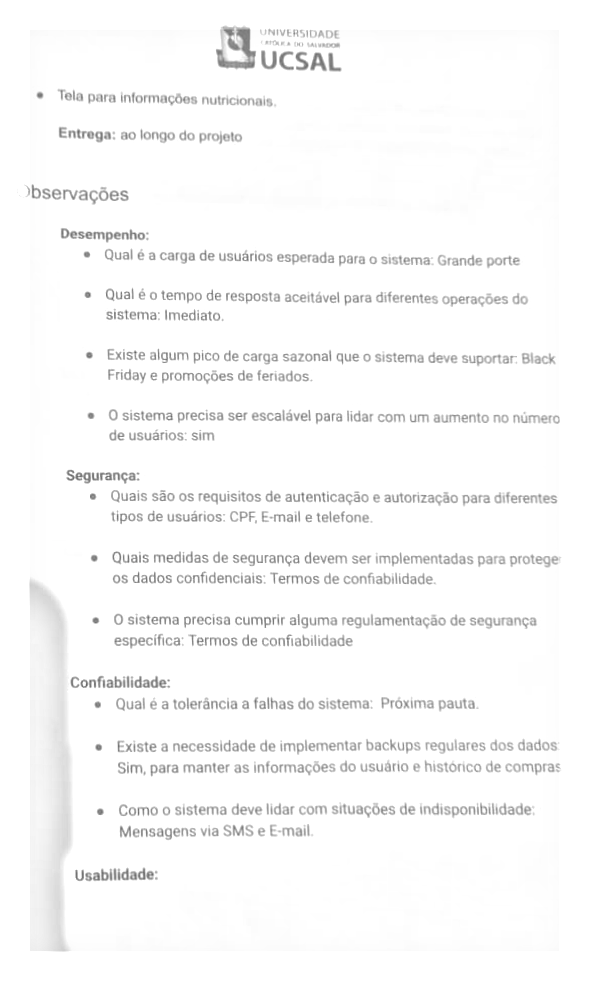
\includegraphics[width=0.75\linewidth]{imagens-template/Entrevista1/Observações.png}
        \label{fig:placeholder}
    \end{figure}
    
    \subsubsection{Assinatura}
    \begin{figure}[H]
        \centering
        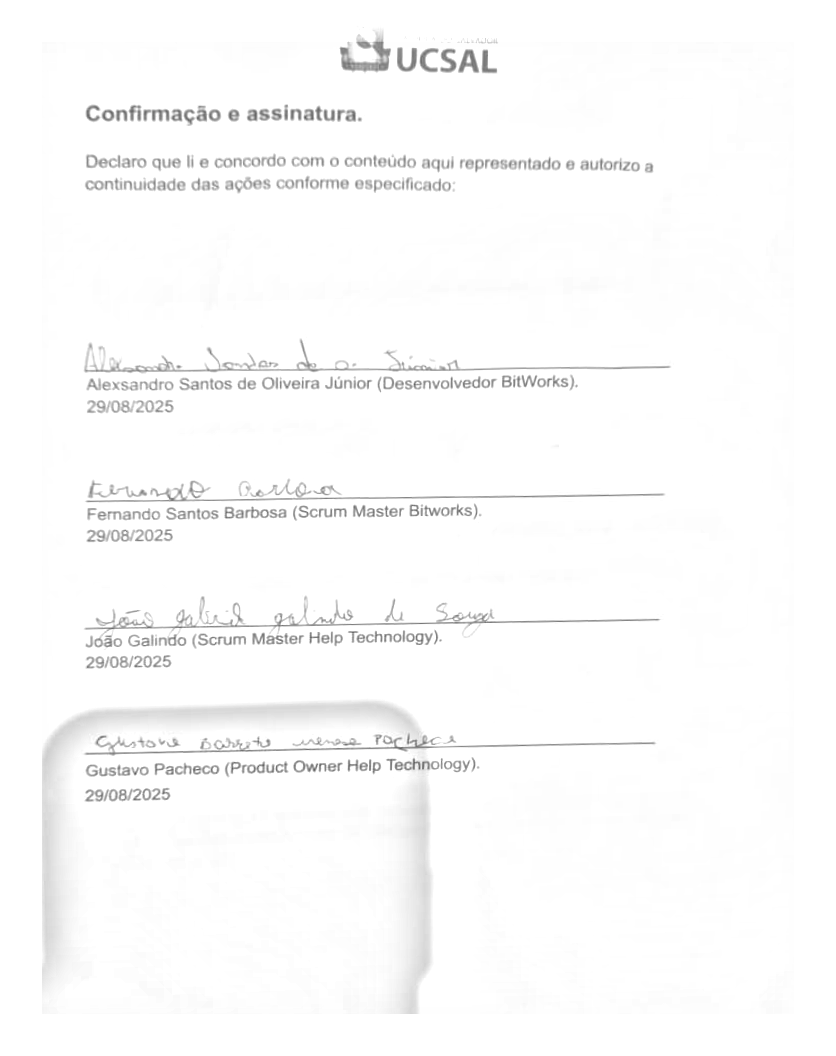
\includegraphics[width=0.75\linewidth]{imagens-template/Entrevista1/assinatura.png}
        \label{fig:placeholder}
    \end{figure}

    %\newpage                                        
    \subsection{Segunda entrevista com o Cliente}
    \subsubsection{Requisitos de Interface Apresentados}
    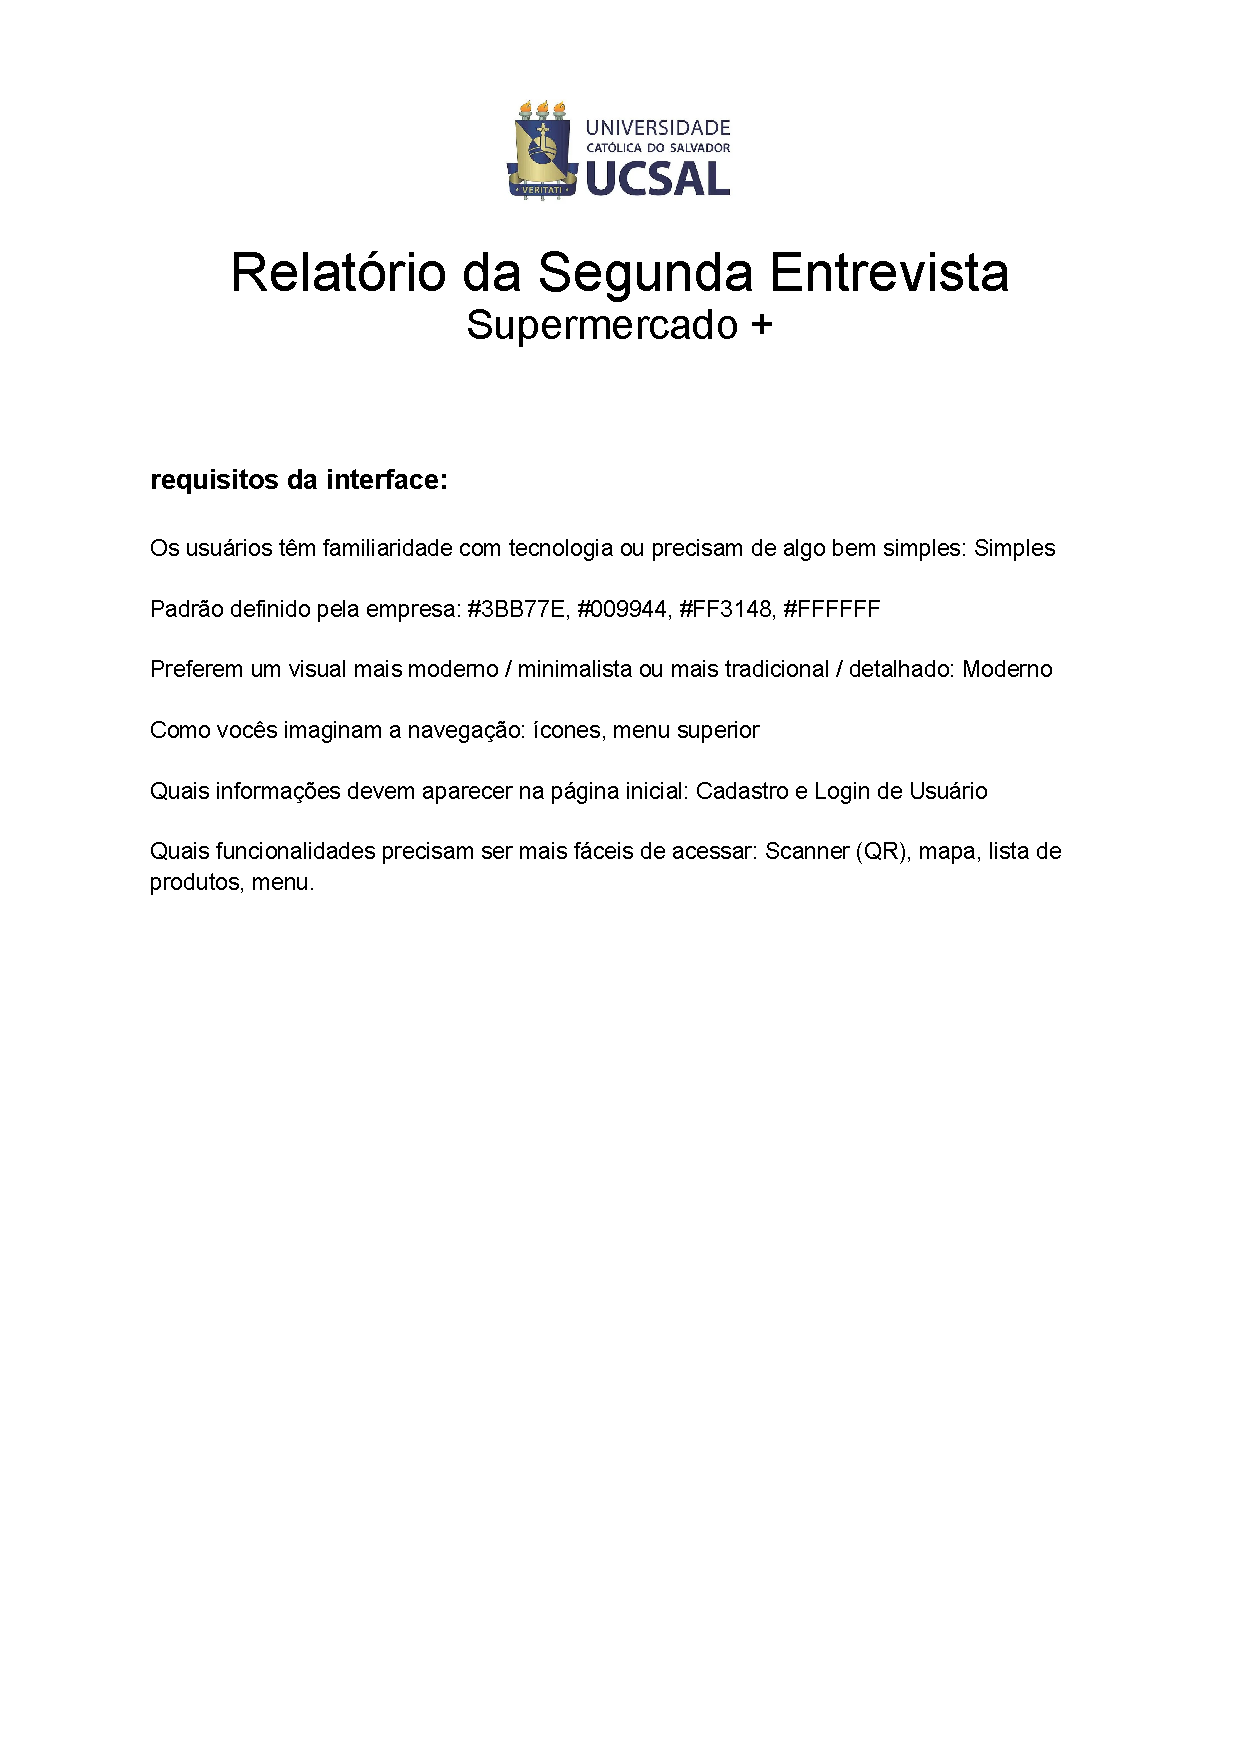
\includegraphics[page=1, width=\textwidth]{imagens-template/arquivos/segunda entrevista.pdf}
    
    \newpage
    \subsubsection{Declaração da Assinatura}
    \includegraphics[page=2, width=\textwidth]{imagens-template/arquivos/segunda entrevista.pdf}
    \subsubsection{Assinatura}
    \includegraphics[page=3, width=\textwidth]{imagens-template/arquivos/segunda entrevista.pdf}
    \vspace{12mm}
    
    %\newpage                                          
    \section {Requisitos Funcionais e Não-Funcionais}   
    \vspace{12mm}                                       
    \subsection{Requisitos Funcionais}
    \begin{itemize}
    \item Permitir cadastro de usuário com e-mail, senha, CPF, número de telefone e CEP.
    \item Permitir login através de e-mail, CPF ou telefone.
    \item Permitir que o usuário selecione supermercados parceiros integrados à plataforma.
    \item Localizar supermercados em tempo real ou por CEP.
    \item Exibir a localização dos produtos dentro do supermercado por meio de mapa inteligente.
    \item Permitir consulta de preços e informações nutricionais via leitor de código de barras.
    \item Exibir preços atualizados dos produtos.
    \item Fornecer informações nutricionais detalhadas de cada produto.
    \item Permitir compras online com opção de retirada no supermercado.
    \item Garantir fácil acesso às funcionalidades principais: scanner (QR), mapa, lista de produtos e menu.
    \item Integrar-se a outros sistemas ou APIs externas, utilizando HTTP/HTTPS (REST APIs) e JMS (Java Message Service).
    \item Suportar múltiplos idiomas configuráveis pelo usuário.
\end{itemize}

    \newpage
    \subsection{Requisitos Não Funcionais}
    \begin{itemize}
    \item Suportar grande carga de usuários simultâneos.
    \item Garantir tempo de resposta imediato para as operações do sistema.
    \item Suportar picos sazonais, como Black Friday e promoções.
    \item Ser escalável para aumento do número de usuários.
    \item Implementar autenticação por CPF, e-mail e telefone.
    \item Proteger os dados do usuário conforme os termos de confiabilidade.
    \item Realizar backups regulares das informações do usuário e histórico de compras.
    \item Notificar o usuário sobre indisponibilidade do sistema via SMS e e-mail.
    \item Interface simples, moderna e de fácil navegação, utilizando ícones e menu superior.
    \item Sistema web responsivo, com possibilidade de futura versão mobile.
    \item Compatível com diferentes sistemas operacionais: Windows, Linux e macOS.
    \item Suportar diferentes navegadores e dispositivos móveis.
    \item Atualizações do sistema realizadas via backups e versionamento.
    \item Garantir confiabilidade e tolerância a falhas do sistema, mantendo integridade das informações.
\end{itemize} 
    
                                
    
    \newpage
    \section{Cronograma (Power-Up) Completo do Projeto e Relação dos Participantes}
    \href{https://trello.com/b/ibXrGxlH/trello-de-desenvolvimento}{\textbf{Clique aqui para acessar o cronograma}}
    \begin{itemize}
         \item Alexsandro S. de O. Júnior – 1 (Contribuiu)
        \item Fernando Santos Barbosa – 1 (Contribuiu)
        \item João Moraes Gordilho – 1 (Contribuiu)
        \item Antonio Victor Azevedo Nascimento de Seixas Rocha – 2 (Não Contribuiu)
        \item Erivelton Madureira Lopes – 2 (Não Contribuiu)
    \end{itemize}
    \vspace{12mm}

    \section{Telas do Figma}         
    \vspace{12mm}

    \subsection{Login}
    \begin{figure}[H]
        \centering
        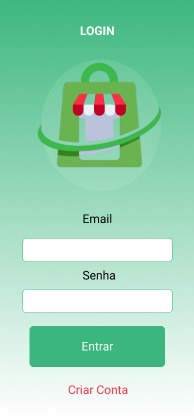
\includegraphics[width=0.5\linewidth]{imagens-template//telas/login.jpg}
        \caption{Enter Caption}
        \label{fig:placeholder}
    \end{figure}
    
    \subsection{Seleção de Mercados}
    \begin{figure}[H]
        \centering
        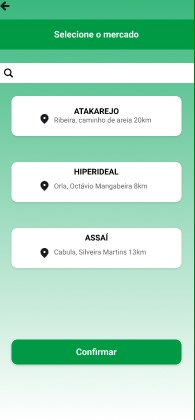
\includegraphics[width=0.5\linewidth]{imagens-template//telas/seleçãoMercado.jpg}
        \label{fig:placeholder}
    \end{figure}

    \subsection{Mapa}
    \begin{figure}[H]
        \centering
        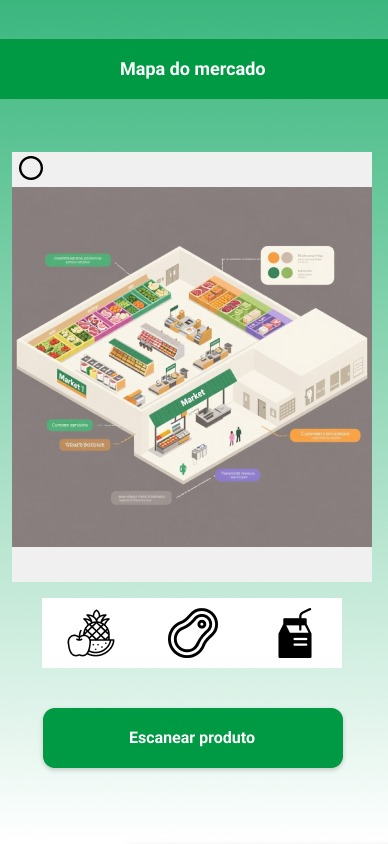
\includegraphics[width=0.5\linewidth]{imagens-template//telas/mapa.jpg}
        \label{fig:placeholder}
    \end{figure}

     \subsection{Produtos}
    \begin{figure}[H]
        \centering
        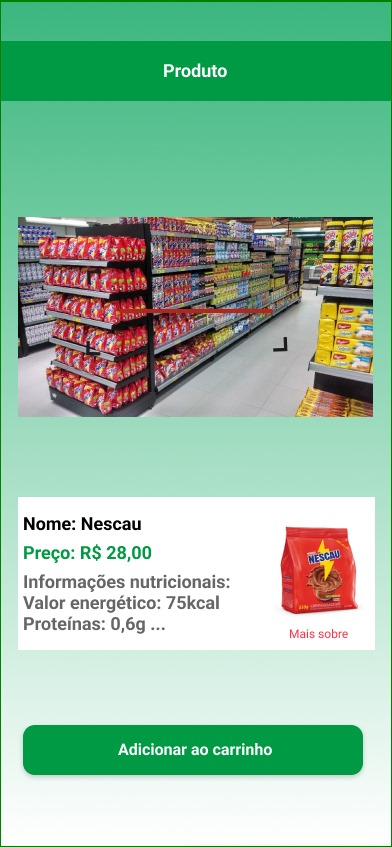
\includegraphics[width=0.5\linewidth]{imagens-template//telas/produto.jpg}
        \label{fig:placeholder}
    \end{figure}
    
     \subsection{Carrinho}
  \begin{figure}[H]
        \centering
        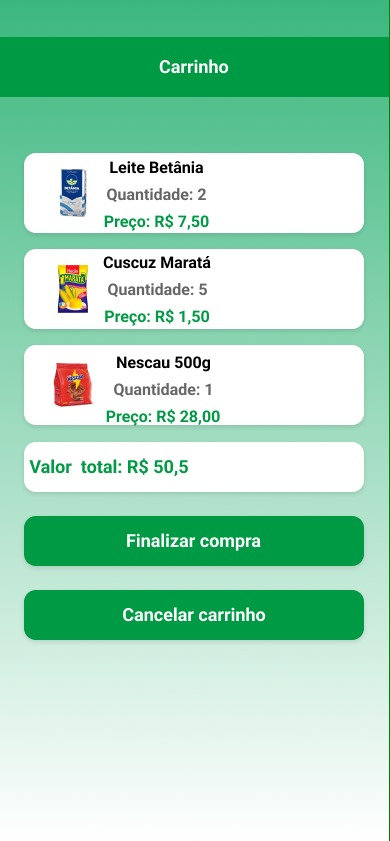
\includegraphics[width=0.5\linewidth]{imagens-template//telas/carrinho.jpg}
        \label{fig:placeholder}
    \end{figure}
    
 \subsection{Retirada}
\begin{figure}[H]
        \centering
        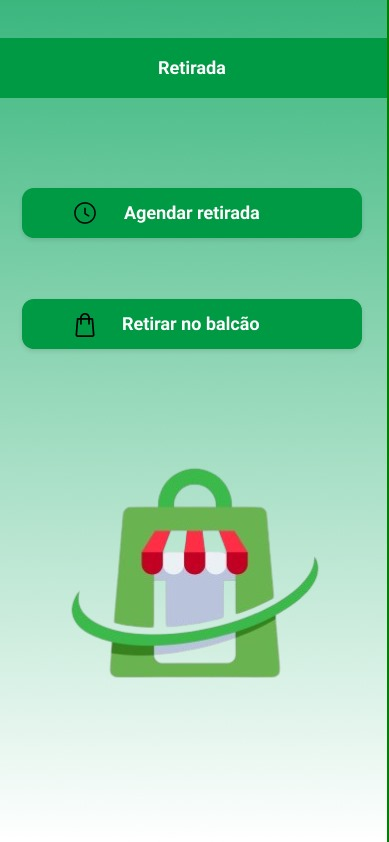
\includegraphics[width=0.5\linewidth]{imagens-template//telas/retirada.jpg}
        \label{fig:placeholder}
    \end{figure}
    
 \subsection{Código de Barras}
   \begin{figure}[H]
        \centering
        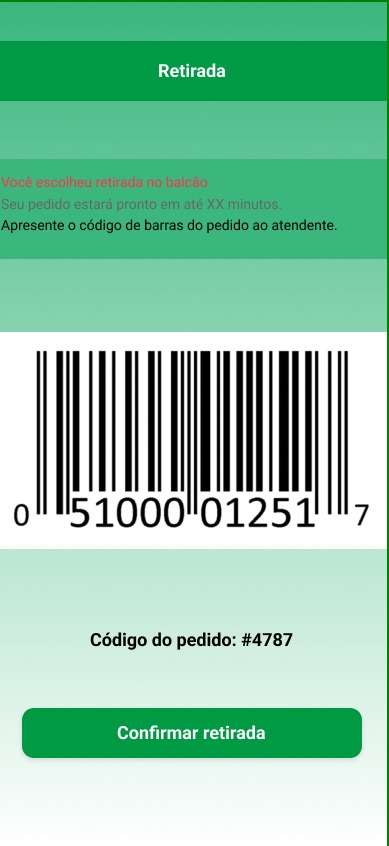
\includegraphics[width=0.5\linewidth]{imagens-template//telas/qrpagamento.jpg}
        \label{fig:placeholder}
    \end{figure}
    
 \subsection{Cadastro de Supermercados}
   \begin{figure}[H]
        \centering
        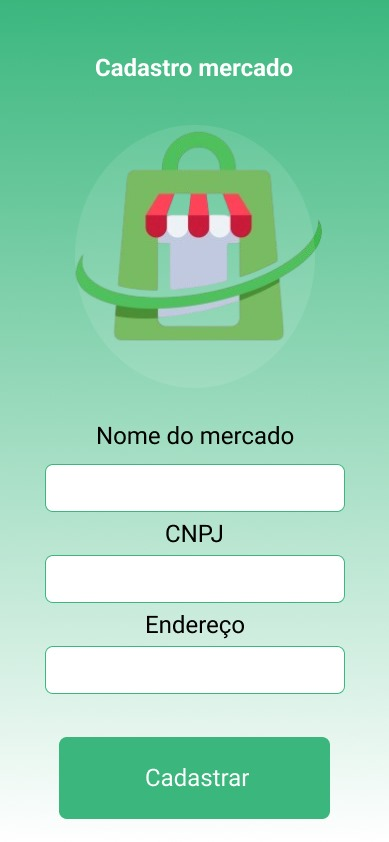
\includegraphics[width=0.5\linewidth]{imagens-template//telas/cadastroSupermercado.jpg}
        \label{fig:placeholder}
    \end{figure}

                          
    \newpage                                        
    \section{Termo de Aceite do Cliente Assinado}
    
\includegraphics[page=1, width=\textwidth]{imagens-template/arquivos/Termo de aceite.docx.pdf}
    \newpage
     
\includegraphics[page=2, width=\textwidth]{imagens-template/arquivos/Termo de aceite.docx.pdf}
      
\includegraphics[page=3, width=\textwidth]{imagens-template/arquivos/Termo de aceite.docx.pdf}
    \vspace{12mm}                                   
                        
\end{document}